%% Template file for all Software/Hardware modules

% Replace "Name of Module" with the name of this module
\chapter{Satellite Prototype}

\section{Description}

The purpose of the Satellite is to measure and transmit the voltage,
and the amount of current being drawn on the particular outlet that 
the Satellite is plugged into. The module is done this way so that
the current and voltage can be measured quickly and efficiently.


\section{Circuit Diagrams}

Figure \ref{MeasuringCircuit} shows the layout of the Satellite's 
measuring hardware. Mains electricity will be run through a current
transformer which will measure only a fraction of the actual current. 
This will be enough to determine how much is actually being drawn. 
We then pass the current through a diode, to ensure that the negative half of the signal doesn't pass. 
The current will go through a sense-resistor and then into an Analog to Digital converter. 
The resistor is in place for troubleshooting. 

\begin{figure}[H]
\centering
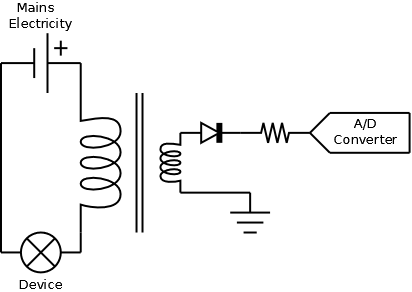
\includegraphics[scale=0.3]{Hardware/images/MeasureCircuit.png}
\caption{Measuring Circuit}
\label{MeasuringCircuit}
\end{figure}

\section{Pinout Diagrams}
Figure \ref{XBeePinout} shows the pinouts of the XBee modules that
we will be using. For this project we will be using pins 1, 2, 3, and 10.
Pin 1 is simply the 3.3V source. Pin 2 is the Data Out and will be 
responsible for talking to the rest of the ZigBee Mesh. Pin 3 is the 
Data In. This pin will be responsible for listening to the ZigBee Mesh.
Pin 10 is ground.

\begin{figure}[H]
\centering
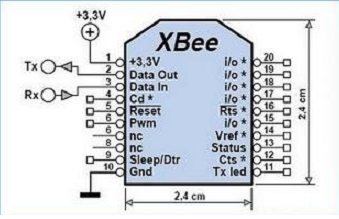
\includegraphics[scale=1.0]{Hardware/images/XBeePinout.png}
\caption{XBee Pinout}
\label{XBeePinout}
\end{figure}

\section{Potential Problems}

% A list of potentional programs along with suggestions
%  on ways to work around them. Elaborate on why the problem
%  exists
We will have to be careful to ensure that the Satellite does 
not catch fire. We are interfacing with 120VAC electricity, and 
this introduces the possibility of electrical fires. 
Safety precautions must be in place to prevent that. 